\chapter{An overview of the Hazel programming environment}
\label{sec:hazel}

Hazel is the reference implementation for the Hazelnut bidirectionally-typed action semantics and the Hazelnut Live dynamic semantics. It is intended to serve as a proof-of-concept of the semantics with static holes that attempt to mitigate the gap problem; however, the implementation is becoming increasingly practical with additional research efforts. The reference implementation is an interpreter written in OCaml and transpiled to Javascript using the \mintinline{text}|js_of_ocaml| (JSOO) library \cite{vouillon2014bytecode} so that it may be run client-side in the browser. A screenshot of the reference implementation is shown in \Cref{fig:screenshot-hazel-ui} \cite{HazelDemo2022}. The source code may be found on GitHub \cite{Hazel2022}. As a programming language, Hazel can be characterized as a purely functional, statically-typed, bidirectionally-typed, strict-order evaluation, structured editor language.

\section{Motivation for Hazel}
\label{sec:hazel-motivation}

\subsection{The gap problem}
\label{sec:gap-problem}

\todo{add citations in this section -- use citations from Hazelnut Live 2019 paper}

Programming editor environments aim to provide feedback to a programmer in the form of editor services such as syntax highlighting or warnings using the LSP. Live programming environments aim to provide continuous static (static type error) and dynamic (run-time type error) feedback in real-time, allowing for rapid prototyping. However, over the course of the lifetime of a program, the program may enter many edit states when it is \textit{meaningless} (ill-formed or ill-typed).

Editor services can only assign static and dynamic meaning to programs that are statically well-typed and free of dynamic type errors. Some may deploy reduced ad hoc algorithms of meaningless edit states. This means that over the course of editing, the programmer experiences temporal gaps between moments of complete editor services. This is known as the \textit{gap problem}.

\subsection{An intuitive introduction to typed expression holes}
\label{sec:typed-holes}

Hazelnut and Hazelnut Live address the gap problem by defining a static and dynamic semantics, respectively, for a small functional programming language extended with typed holes. It is built on top of a structure editor, which ensures that a program is always well-formed (syntactically correct). The Hazelnut action semantics for typed holes ensures that a well-formed program is always well-typed. The Hazelnut Live dynamic semantics defines an encapsulated behavior for type errors, such that evaluation continues ``around'' and captures information about type errors in order to provide dynamic feedback to the programmer.

The Hazelnut Live paper provides the following intuitive understanding of holes.

\begin{displayquote}
  Empty holes stand for missing expressions or types, and non-empty holes operate as ``membranes''
around static type inconsistencies (i.e. they internalize the ``red underline'' that editors commonly display under a type inconsistency).
\end{displayquote}

We have already acknowledged the existence of type holes in dynamically-typed languages and in the \gtclc{}, in which type holes are represented by the type $\gtlch$. This allows unannotated expressions to statically type-check, with the possibility of running into a dynamic type error at runtime.

Some languages also have the concept of expression holes, which allow a program to be well-typed with missing expressions. In Haskell, for example, the special error value \mintinline{haskell}|undefined| always type-checks but will immediately crash the program if it is encountered during evaluation. Haskell also provides the syntax \mintinline{haskell}|_u| for expression holes \todoref{cite this}, which provides static type information but will not successfully compile. The mechanism to insert expressions holes may be either automatic or manual \todoref{cite this}. However, no such example of expression holes have a well-defined dynamic semantics that allows continuation past the hole with useful feedback \todoref{cite this -- perhaps cite hazelnut 2019 paper}.

In summary, Hazel provides empty type and expression holes, which represent dynamic typing and missing expressions. Nonempty holes are also provided to encapsulate error conditions and provide a well-defined dynamic semantics while providing useful feedback to the user. The dynamic semantics is carefully defined to stop when such indeterminate expressions are encountered, but continue elsewhere (``around'' holes or failed casts) if possible.

\subsection{The Hazel interface}
\label{sec:hazel-interface}

In \Cref{fig:hazel-interface} the web interface for the Hazel live environment is shown. The left panel marked (1) is a informational panel showing the list of keyboard shortcuts to perform actions. Since Hazel is a structured editor, simply typing the program as plaintext will not work; one must use the appropriate shortcuts the construct and edit the program. (2) is the code view. Below the code, a gray box indicates the result of evaluating the expression. The program result updates in real time with every edit action, assuming that evaluation is turned on. (3) is the context inspector, which shows information about a hole if a hole is selected. It shows the hole environment and typing context, followed by the path to the hole and the number of hole instances. In this case, the third hole in the result is selected, in which $x$ has value $3$. Lastly, (4) shows a history of the edit actions. Hovering or clicking on a past edit state will revert the program to that edit state.

\begin{figure}
  \centering
  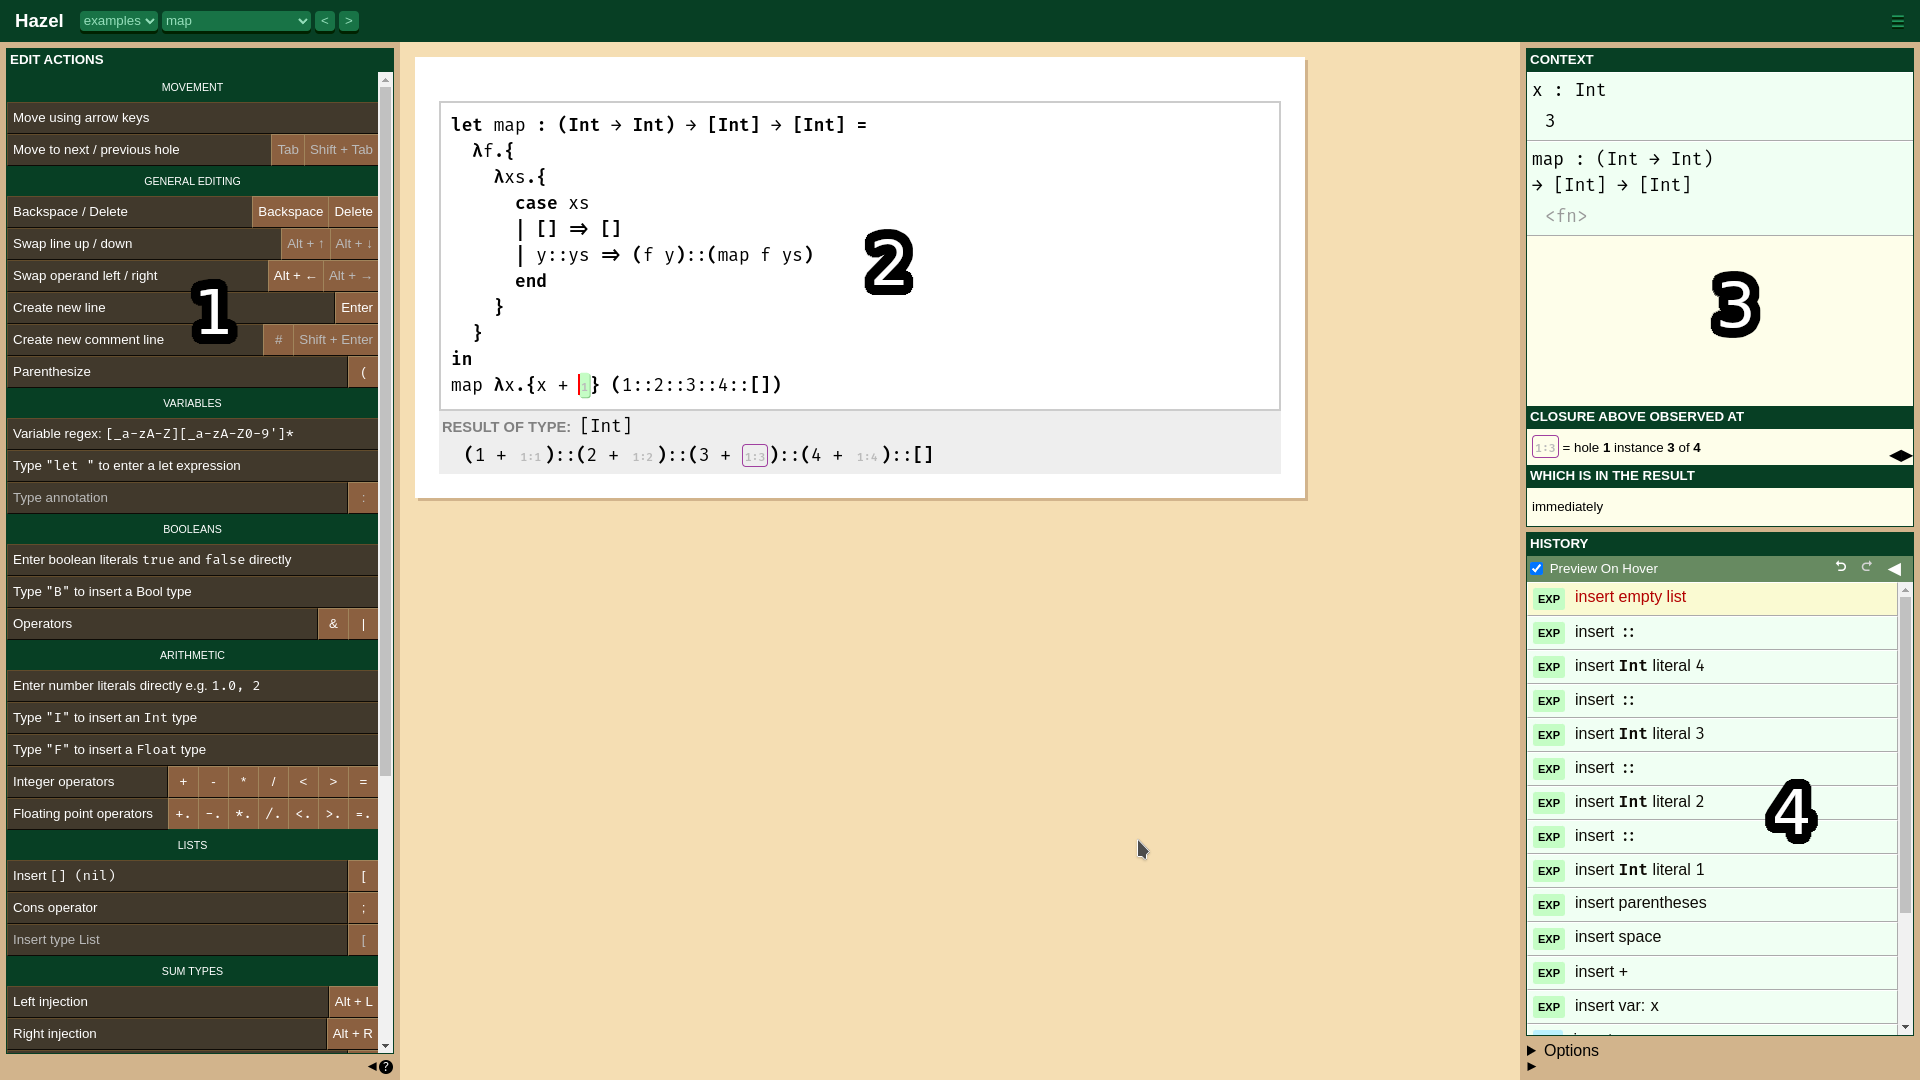
\includegraphics[width=\linewidth]{img/hazel_ui_annot.png}
  \caption{The Hazel interface, annotated}
  \label{fig:hazel-interface}
\end{figure}

\subsection{Implications of Hazel}
\label{sec:hazel-implications}

The main proposed use case of Hazel is its use in programming education, particularly for teaching functional programming, as it provides much useful feedback to the programmer for error conditions, allowing them to focus instead on semantic errors in their algorithm. This is being explored with the Hazel Tutor project \cite{potter2020hazel}.

Another research direction is in its use as a structural and graphical editor. For example, live GUIs \cite{omar2021filling} are being explored to enhance the editing experience by providing live, compositional, graphical interfaces, in addition to the benefits that Hazel's core calculi provide.

The result of a Hazel evaluation may contain holes, and thus not be fully evaluated. The Hazelnut Live paper \cite{conf/popl/HazelnutLive19} suggests the idea of hole-filling: since each hole in the result contains its lexical environment, we may ``resume'' evaluation without restarting evaluation from the beginning if a hole is filled. An interesting application of this is in the use of notebook-style programming editors such as Jupyter Notebook \todoref{citation} and MATLAB \todoref{citation}, which are common in scientific computing \todoref{citation}. Notebook-style editors are useful because they allow evaluation of sections of a script, usually to avoid recomputation of previous sections. The problem is that notebook execution is stateful and running operations out-of-order will cause irreproducible results. On the other hand, resuming an evalution with fill-and-resume will produce the same result as if the program was run ordinarily from start to finish\footnote{This is a property known as \textit{commutativity} and described in \cite{conf/popl/HazelnutLive19}.}.

\section{Introduction to OCaml and Reason}
\label{sec:ocaml-intro}

Previously, we have been introducing concepts using a pseudo-mathematical notation. Henceforth, when describing Hazel and its implementation, it may be useful to use sample code or pseudocode from the implementation to describe various aspects of Hazel.

Hazel is implemented in Reason, which is a dialect of OCaml. Except for code samples in \Cref{app:code-samples}, the notation used throughout this report will be limited to referring to function names and types. Module names are denoted \texttt{}PascalCase, whereas function and type names are \texttt{snake\_case}. Conventionally, modules that export a type export a single type called \texttt{t}. As an example, \mintinline{ocaml}|DHExp.t| refers to the primarily-relevant type from the \mintinline{ocaml}|DHExp| module, the type that represents internal expressions $d$. On the other hand, \mintinline{ocaml}|Evaluator.evaluate| refers to the \mintinline{ocaml}|evaluate| function in the \mintinline{ocaml}|Evaluator| module. All functions and types will be prefixed with their module names for clarity.

\section{Hazel semantics}
\label{sec:hazel-semantics}

\subsection{Statics: Hazelnut action and typing semantics}
\label{sec:hazel-statics}

\subsection{Dynamics: Hazelnut Live dynamic semantics}
\label{sec:hazel-dynamics}

The internal language is highly similar to the external language. The primary difference is the introduction of the cast calculus taken from the GTLC described in \Cref{sec:gradual}. Practically, there is also the introduction of the fixpoint to allow for recursion, as the fixpoint is not exposed to users in the external language.

\textit{Elaboration} is the process of converting an expression from the external language to the internal language. Notably, both the external and internal languages share the same type system.

The elaboration algorithm is bidirectionally-typed, and thus involves two mutually-recursive judgments: a \textit{synthetic elaboration judgment} $\Gamma\vdash e\Rightarrow\tau\leadsto d:\tau\dashv\Delta$, and an \textit{analytic elaboration judgment} $\Gamma\vdash e\Leftarrow\tau\leadsto d:\tau'\dashv\Delta$. $\Delta$ is the \textit{hole context}, used to store the typing context and actual type of each hole, and is an output of the judgments. As with bidirectional typing, the synthetic judgment outputs the synthesized type alongside the elaborated internal expression $d$; the analyzed judgment takes a type $\tau$ to analyze against, and returns the elaborated internal expression $d$ along with its actual type $\tau'$. Having the actual type of analyzed expressions is useful for generating dynamic casts as described in the GTLC.

\subsection{Hole instance numbering}
\label{sec:hole-instance-numbering}

\todo{implement this section}

%%% Local Variables:
%%% mode: latex
%%% TeX-master: "main"
%%% End:
